\begin{problem}{五星珠}{五星珠.in}{五星珠.out}{1.5 seconds}


农夫Pi正在给他的栅栏刷油漆。

栅栏由$n$根竖直木条组成,从左到右第$i$根木条的高度为$h_i$米,宽度为1米。

即,可将第$i$根木条视为坐标轴上四个顶点为$(i-1,0),\ (i,0),\ (i,h_i),\ (i-1,h_i)$的矩形。

Pi的刷子宽度正好为1米,平时他的刷法是对每根木条竖直刷一次来保证完全覆盖,他发现适当地横向刷漆可以减少工作量。

因此这次他可以选择横着刷或竖着刷,但是刷子必须全程保持在栅栏上(见样例解释获取更多信息),粉刷过的地方可以被重复粉刷。

\InputFile

第一行一个整数$n\ (1\le n\le 5000)$

第二行$n$个整数$h_1,h_2,\cdots,h_n\ (1\le h_i\le 10^9)$

\OutputFile

一个整数,表示将栅栏整体粉刷完成最少所需的次数

\Example

\begin{example}
\exmp{
12
10 10 1 1 1 3 3 3 3 3 3 3
}{
5
}%
\exmp{
1
5000
}{
1
}%
\end{example}
\\
对于样例1,可以先粉刷最底层(粉色1次),之后竖直粉刷最左侧的高度为10的2根木条(黄色2次),之后再横向粉刷右侧高度为3的木条(蓝色2次)。

见下图,左下角被重复粉刷。
\begin{center}
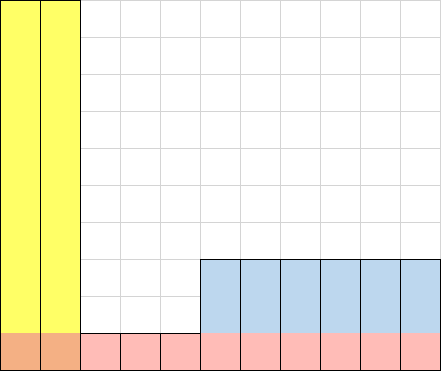
\includegraphics[width=0.4\textwidth]{pics/E.png}
\end{center}
\end{problem}
